\chapter{Schedule Replication}
In chapter ~\ref{chap:detexec} we described using a deterministic system to ensure the applications on the primary and secondary replica can have the same thread interleaving. The major advantage of the deterministic system is that we can minimize the communication between the replicas. However the downside is that we need to precisely adjust the logical time to maintain decent parallelism for multithreaded applications. We showed various solutions to balance the logical time because we need to keep the execution to be deterministic. If all the burdens come from being deterministic, can we break the determinism once for all but still keep the replicas to be deterministic? The answer is yes.

In this chapter we are going to describe Execute-Follow model for replicated applications. In this algorithm, we break the determinism entirely and use messages to synchronize every single synchronization primitives between the primary and replica. This chapter is organized as follows:

\begin{itemize}
  \item In blah we describe blah
  \item In blah we describe blah
\end{itemize}

\begin{figure}
\centering
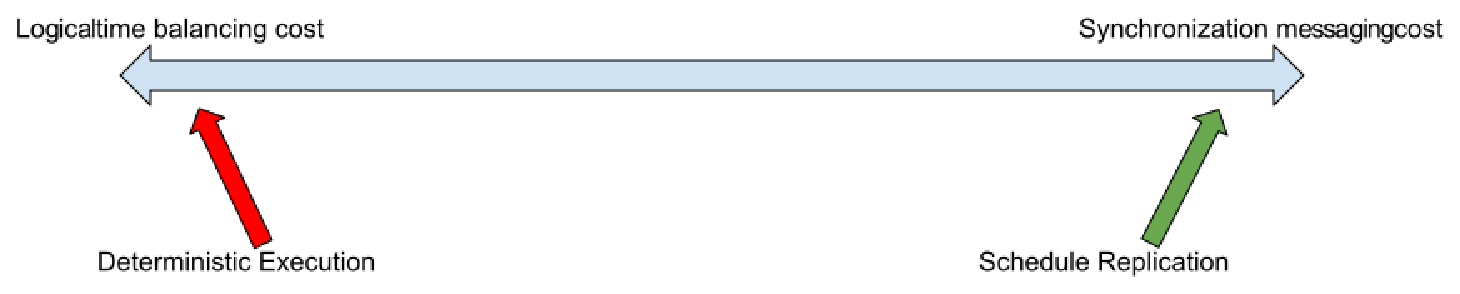
\includegraphics[width=0.8\columnwidth]{figures/tradeoff}
\caption{Trade off between two algorithms}
\label{f:tradeoff}
\end{figure}
\section{Execute-Follow Model}
\section{Implementation}